\documentclass[pscyr, 12pt]{hedlab}
\usepackage[russian]{babel}
\usepackage{graphicx}

\graphicspath{{images/}}

\labname{Разработка баз данных в СУБД Oracle}
\labnum{5}
\student{Голубев~А.~В., САПР-1.1п}
\labdate{}

\begin{document}
    \makeheader
    \noindent\textbf{Цель:} создание формы вывода данных

    \noindent\textbf{Постановка задачи:}
    \vspace*{-1em}
    \begin{itemize}\itemsep-5pt
        \item изучить функциональные возможности программы
        \item создать форму для данных
        \item вывести данные в форму
    \end{itemize}

    Используем мастер \emph{Block Wizard} для создания формы
    \begin{figure}[ht!]
        \center
        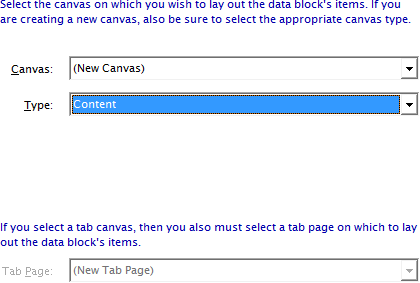
\includegraphics[width=0.47\textwidth]{lab05_01}
    \end{figure}

    Выбираем элементы таблицы для вывода
    \begin{figure}[ht!]
        \center
        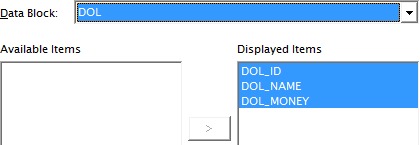
\includegraphics[width=0.47\textwidth]{lab05_02}
    \end{figure}

    Определяем поле \emph{promt} для каждого элемента
    \begin{figure}[ht!]
        \center
        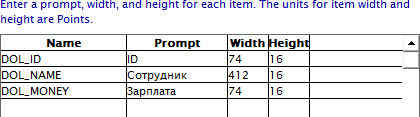
\includegraphics[width=0.47\textwidth]{lab05_03}
    \end{figure}

    \pagebreak

    Устанавливаем заголовок и количество отображаемых элементов
    \begin{figure}[ht!]
        \center
        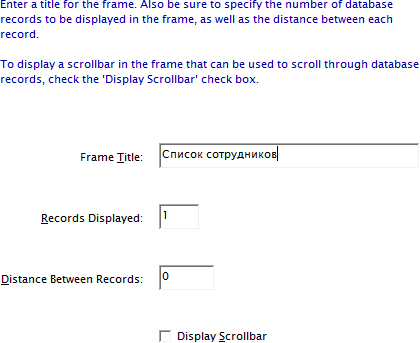
\includegraphics[width=0.6\textwidth]{lab05_04}
    \end{figure}

    Результат запуска
    \begin{figure}[ht!]
        \center
        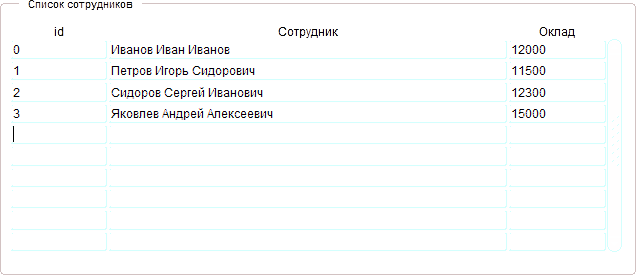
\includegraphics[width=0.8\textwidth]{lab05_05}
    \end{figure}

    \noindent\textbf{Вывод:} в результате проделанной работы
    \vspace*{-1em}
    \begin{enumerate}\itemsep-5pt
        \item создана форма для вывода информации
        \item выведена информацию из БД в созданную форму
        \item изучен базовый функционал программы
    \end{enumerate}
\end{document}